\chapter{The Vision of Soft Buildings}

We begin with a vision for the future of buildings.  We would like to turn all buildings into ``smart''
buildings that provide services to its occupants, the grid, and the environment.  Currently, buildings
are largely built in isolation of one another -- each unique in its own right, from the material the walls
are made of to the systems and software that control them.  With the falling cost of memory, the ubiquity of
connectivity and sensing, and cheap cost of computation in the cloud, it should be possible to make buildings ``smarter''
through software guided by the principles of extensibility and clean, well-defined software interfaces.

We would like to move towards a vision of building software systems that

\begin{enumerate}
\item Support the notion of applications; applications to make use of and directly control the environment.
\item Provide a clean set of abstraction for application writers that wish to build both analytical and control
applications.
\item Accurately capture the state of the building, even as it evolves.
\end{enumerate}


Recent trends in research and technology set the stage for our work.  We give a brief history of the work that has 
led us to the vision of a smart built environment.  We also describe the technology that
allows us to realize our vision and show how the falling cost of sensor, ubiquity of connectivity and embedded computation,
and falling cost of computation in the cloud informs our architectural choices.
In the next section, 
we discuss the built environment and how energy-efficiency has become a prime research focus.
Then, we give an overview of pervasive computing work and explain how they motivate the kinds of applications we look 
to support in the built environment.  Finally, we will state our research goal and give an overview of the rest
of the thesis.




\section{The Built Environment}
Humans spend a large portion of their lives in buildings and
there are known problems related to energy consumption, comfort, and operational visibility.  
Buildings consume 40\% of the energy produced in the United States and nearly three quarters of 
the electricity produced~\cite{epabuildings}.  With specter of global warming and the continued decrease in the cost of storage and 
communication, buildings have become a major target for improved energy efficiency.

Buildings have been the subject of study for architects, mechanical, and building engineers.  Recently, there has been an 
interest in buildings by computer scientists as they present a family of interesting challenges related to cyber-physical systems.
Historically, building manangers and contractors work together with a third-party provider to embed sensors through the systems
and spaces in the building to allow them to observe and manage
the day-to-day operations of the building from a central location.  The building manager is the primary user to interact with the
deployment information to diagnose and fix problems from a central locations.  Problem identification primarily occurs through occupant 
complaints.  The building manager diagnoses through physical inspection and simple inspection of the associated data through the primary
user interface for the \emph{building management system}.  These BMS's are common in large buildings.
Over 70\% of large -- 100,000 square feet or larger -- commercial buildings, have a building management 
system~\cite{cbecs2003}.  These systems are installed primarily for supervisory control and
centralized observation of the building.  
They help deal with the management complexity and supervisory control of a highly distributed mechanical system through
a graphical view and the sensors and actuators they contain.



% We assert that live and historical 
% sensor data must be exposed to application developers so they may build application that easily and continuously 
% asses the state of the building, identify faulty behavior, and enable holistic control.  


% We envision a future
% where buildings provide a standard way to observe and assess their operational performance, supports 
% the broad notion of programmability and enables the creation of different building applications, and 
% allows supports the suite of tools currently available for analyzing and controlling
% it.  We hope that future and to support emerging technologies that enhance these tasks.
% % We consider technological trends that set the stage
% % the work discussed in the thesis.  
% We examine problems in building with respect
% to energy efficiency and system maintenance and explore how computing can help. 


%   In order to optimize building performance, we need fine grained visibility into the energy flow
% throughout the building.  

% However, if you examine the infrastructure currently in place to provide this visibility you will discover tightly 
% integrated silos, bloated interfaces, and a lack of extensibility that is necessary to support broad 
% application development.  
\begin{figure}[h!]
\begin{center}
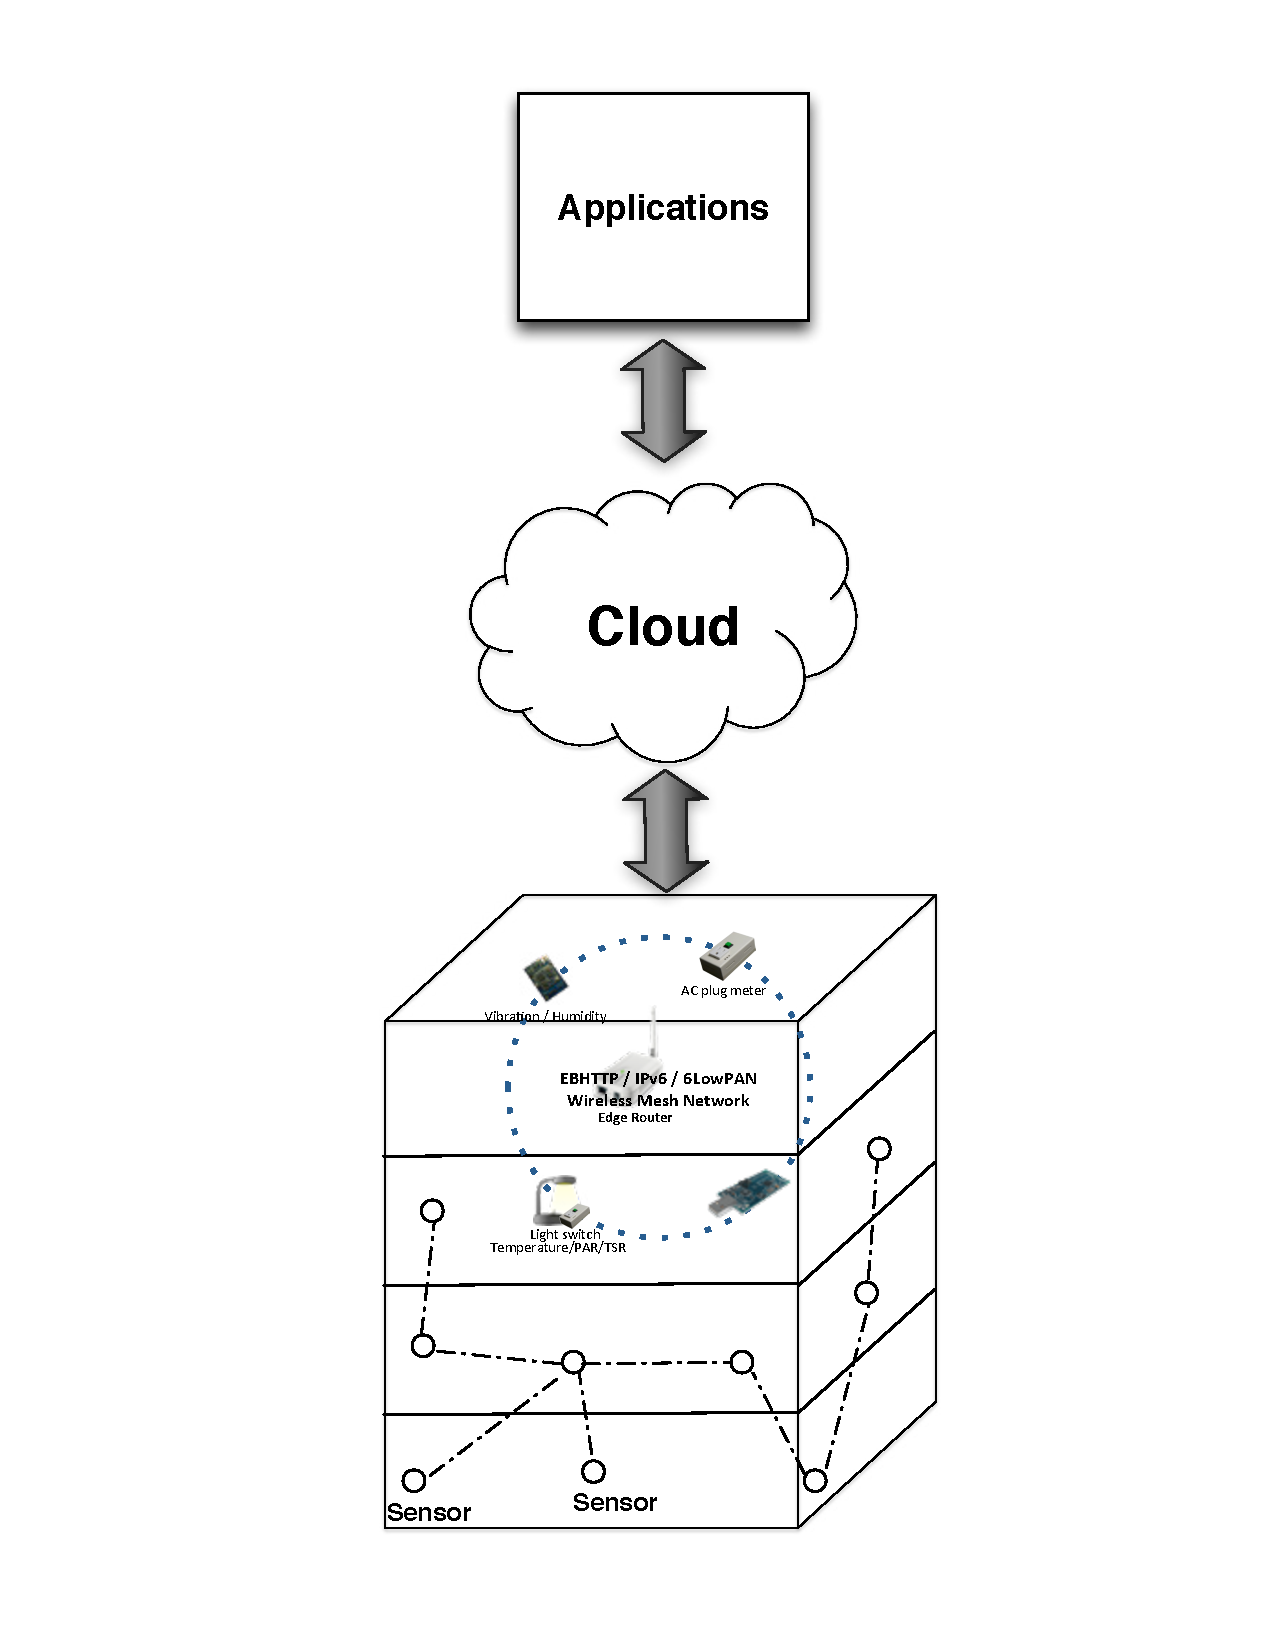
\includegraphics[width=0.5\textwidth]{figs/BuildingAppModel}
\caption{Building application model.  Building sensor deployments send data to the cloud and applications access it as it streams in.
Applications may also feed data to the cloud and make it available to other applications.}
\label{fig:buidlingapp}
\end{center}
\end{figure}



\section{Pervasive Computing}
The proliferation of cheap, networked, embedded sensors is moving us towards a future where our infrastructure is 
populated with computing that enable smart environments.  We march towards Mark Weiser's vision of the future of
computing \cite{uqicomp_vision} where the environment contains sensors and people interact with the 
physical environment through their personal devices and related services.  These services also allow us to 
optimize the performance of our infrastructure, uncover problems proactively,
and share information with others to provide greater insight into the world around us.  
% This vision is borne out
% incrementally in the research community over the past 20 years.%since the vision was initially proposed over 20 years ago.

The research in this area starts from the vision for the field.  What could the world be if we are surrounded by computing?
How will we interact in that world?  What can we learn from the world and from each other?  Hypothetical scenarios
guide the early work.  A common scenario is one that makes use of a personal handheld device, ``smart'' objects, and 
ubiquitous connectivity.  Much of the early work aimed at constructing a scenario that captures some aspect of
the future envisioned that can be used to highlight and explore fundamental challenges in realizing the vision.
For example, Christensen et al.~\cite{Christensen_2002} explore how pervasive computing will play a role in assisting
office workers in their day to day activities.  They imagine a scenario where office occupants use their mobile devices
to interact and share information with each other through serendipitous work-related activities.  Through this scenario
draw attention to fundamental issues related to mobility, interrupted operations, and activity scheduling.% due to ad-hoc 
% collaboration.

Many fundamental challenges were discovered and addressed in this fashion.  Pervasive computing work eventually branched
off into several sub-domains with their own focus.  Some examples are work related to 
localization~\cite{Castro01aprobabilistic,Koo,Romer03thelighthouse,Yoon2013}, 
mobility and mobile devices~\cite{Haritaoglu:2001:ILR:647987.741331,Want02thepersonal,Jiang:2011:MPM:2030112.2030150},
context deduction and wearable computing~\cite{Holmquist01smart,Lukowicz2002,Christensen_2002,Rossi:2011:RWC:2030112.2030238},
and sensor networks~\cite{Conner:2001:MEL:647987.741329,Lymberopoulos09amethodology}.  These and related
topic areas have guided our thinking in addressing the problems in the built environment.

Looking back at the pervasive computing work, we observe that much of the work has focused on users but not as much on 
the challenges in the environment itself.  There is little
emphasis on the infrastructure and issues with the accuracy in contextual representation of the physical environment.
There is also very little work on how a changing physical environment affects the accuracy with which applications can 
deduce the state of the world around them.  Also, there is very little emphasis on control of the physical environment.
The kinds of software processes that runs in buildings are primarily for control of the environment.  These issues
are neither addressed in the building science community nor the pervasive and computer science community.  We look at these
issues specifically in this thesis.


% Through the construction of vision-style scenarios and application development in those settings, 
% frameworks emerged and fundamental challenges were uncovered. 
% The challenges and solutions are related to localization, contextual inference, multi-modal input, vision, and other issues.
% Eventually each of these branched off into individual fields of study and communities that examined these
% more deeply.
% As these communities matured they were driven by more realistic deployment and application contexts.
% Over the years, this evolution has included advances in sensing, mobile, and network technology but also computational 
% ubiquity through cloud computing.  Moreover, as we consider problems that emerge in specific application domains or
% industries, we will see that the convergence of these technologies allow new domain-specific problems and solutions 
% to be explored.


% Much of the work in computing in the built environment comes from pervasive computing.  Over the last
% 20 years, researchers have explored how computation can be used to capture the physical environment and
% how applications can be used to combine computational resources into a coherent service for users.
% Localization is a fundamental issue addressed~\cite{Castro01aprobabilistic,Koo,Romer03thelighthouse,Yoon2013}.


% % \begin{itemize}
% % % There has been much emphasis on wearable~\cite{} and mobile computing~\cite{}
% % \item Applications for connected devices
% % \item Infrastructure and tools (the environment advertises services, devices compose them and present them)
% % \end{itemize}
% Smart Objects, Context Awareness, Wearable~\cite{Holmquist01smart,Lukowicz2002,Christensen_2002,Rossi:2011:RWC:2030112.2030238}

% Sensor networks~\cite{Conner:2001:MEL:647987.741329,Lymberopoulos09amethodology}.

% Mobile devices and mobility~\cite{Haritaoglu:2001:ILR:647987.741331,Want02thepersonal,Jiang:2011:MPM:2030112.2030150}.

% Much of the work has focused on user but not as much on the challenges in the environment itself.  There is very little
% emphasis on the infrastructure and issues with the accuracy in contextual representation of the physical environment.
% There is also very little work on how a changing physical environment affects the accuracy with which applications can 
% deduce the state of the world around them.  Also, there is very little emphasis on control of the physical environment.
% One of the primary kinds of software processes that runs in buildings are for control of the environment.  These issues
% are neither addressed in the building science community nor the pervasive and computer science community.  We look at these
% issues specifically in this thesis.


% What's lacking?
% > Little to no emphasis on the infrastructure that is already there for collecting informationa about the environment.
% > All the work is human-centric with general components.
% > No emphasis on issues with the data itself and how we can infer context while the context is changing in the physical infrastructure itself.
% 	> No talk about controlling the environment.  Mainly a focus on provided context-deducing/aware middleware and applications.


\section{Cloud Computing, Ubiquitous Connectivity, and Mobile Phones}
Cloud computing has changed the way we design systems that bring together the physical and computational world.  Coupled with the 
continued maturation of networking technologies -- both indoors through Wifi and outdoors through cellular -- and the explosion of mobile
phone use, today's systems are designed with the mobile phone as an access tool for information in the cloud.  It is mostly safe
to assume that this information will be accessible.  Moreover, connection speeds can reach up to 300 Mbps, so serving sophisticated
applications from the cloud and designing them in a highly interactive manner is commonplace.  The main bottleneck is the form of interaction, which
is still a challenge given the small screen of a mobile phone.

These technologies also make it easier to design centrally managed, globally accessible systems.  % into a single system that is centrally accessible.  
Services in the cloud
can serve many clients simultaneously, proving a unified view of the state of the service and the objects in it.  There is little difference 
between the desktop application and the mobile application, other than service presentation.  Moreover, all the data lives \emph{in} the cloud 
and is fetched \emph{from} the cloud by all clients.  The cloud service mediates interaction between all
participants in the system.

\section{Applications in Buildings}
% Advancements made in the pervasive computing communities, trends in technology, and problems in buildings lead us to thrust of this thesis.
We introduce the notion of building ``app-ification''.  Technology enables mobile phone ``apps''; mobile
applications that closely interact with content in the cloud.  We assert that a good way to address problem in the building
by opening up the building's sensor data streams and buildings services that make use of that data.  A system should provide 
\emph{uniform access} to the data and \emph{facilities for cleaning and aggregation}.  It should be \emph{extensible}
so disparate systems could join and share information that could enable new kinds of applications.  Figure~\ref{fig:buidlingapp}
illustrates a high-level of building ``app-ification architecture''.

Building-scientists and architects use a family of products and software packages that take building data 
and analyze it.  We need to support those as well.  The main idea is to expose building sensor streams and related information for 
applications through the cloud.  This allows us to adopt application development design patterns and inherit the benefits of 
centralized management.   It also provides an environment where a diverse set of applications and solutions can be designed
and tested to address fundamental challenges in building management and control.  %and a system where innovation can take place.
% We believe that the cloud-based service model would be effective.  
Such service should offer a data-processing primitives as well.   It should mediate access to sensor data and actuators.
The system should provide support holistic control applications that combine disparate data sources through the service itself.
We describe the design of such a system in Chapter~\ref{chap:SensingInBuiltMain}.

Privacy is a major concern as we consider the ``app-ification'' of buildings.  Detailed information about energy usage can reveal 
information about the activity in the building and can be used to predict the behavior or individuals and organizations.  For example, 
right before a product launch, employees typically spend longer hours at work.  This could be used by a rival company to acticipate
the release of a new product.  Individual usage data can be used by thieves to indicate when a particular occupant is home and what their
move patterns are.  We only partially address the topic in this thesis,
through mechanisms in our architecture that allow the user to control access to individual and aggregate pieces of information.
However, privacy is a much broader topic and there are many techniques available for adoption.  We leave this exploration
for future work.


\section{Research Statement And Hypothesis}
We formally state the thesis that guides our work: %research thesis and hypothesis:
% \emph{What are the architectural components and technical challenges in the design of an information system
% that enables new and supports old classes of applications in the built environment?}  
\emph{How can we incorporate filesystem and database constructs and what are the technical challenges in a system that supports applications
in the built environment?}
Given the emerging applications in
the built environment it is clear that the old information system design is not sufficiently open, flexible, nor
scalable enough to support them.  Old information systems are tightly integrated from the field-level sensor to
the central supervisor control system.  There are two integration points in traditional systems that we argue 
are either fundamentally flawed or insufficient for emerging applications.  We describe the components that 
currently exist and identify those that are missing.  We show how these components/services enable emerging applications.  We also
discuss the technical challenges that must be solved in order to provide the correct semantics for these services.
Furthermore, we discuss a component that is fundamental for providing correct information to applications 
and formalize the notion of verification in the context of the built environment.  We provide several algorithmic 
solutions to these problems, which lay the foundation for a fundamental service in the broader architecture.


\section{Thesis Roadmap}
In the next chapter, we discuss building information systems today.  We dive into their architectural components and introduce some terminology
used in the building space.  We also describe the motivating scenario that they were built for and examine how well the architecture 
can support the ``app-ification'' of buildings.  We give examples of specific applications that we would like to support
and walk through the components that are useful for this purpose and those that are missing.  We propose a set of necessary
components in an architectural re-design that could provide the same support as BMS's today as well as the emerging ones that we
describe and argue that this should be the design of a \emph{building appification system}.

In Chapter~\ref{chap:SFSArchMain}, we give an overview of a system that contains the components we propose in the previous
chapter.  The name of the system is StreamFS.  StreamFS is a cloud-based service that combines filesystem and database constructs
to organize the streaming sensor data, clean and process streams, and provides a unified access layer.
%  for both physical information
% and actuation channels in the physical world.  
We discuss the overall structure each component in the architecture and how they interact with one another.

Chapter~\ref{chap:mechanisms} dives into the details for the components and mechanisms in StreamFS.
Section~\ref{sec:promngt} focuses on the process management component in StreamFS.  The process management component
manages the streams and the processes that consume those streams.  It is designed to support processes that are specified by the user
and managed by StreamFS as well as integrating external processing components and representing them through the file system in StreamFS.
We discuss some of the challenges and present some solutions to a scheduling problem related to providing fresh data  to processing jobs.
We also describe how various kinds of aggregation can be performed on the data, using the filesystem and pipe abstraction
presented and managed by this component.
Section~\ref{chap:naming} discusses how we represent the world as a collection of files.  StreamFS follows the Unix filesystem principle 
where everything is a file and this allows us to provide a unified management layer for the entire set of building deployment
data and metadata.  We discuss the individual file types that we support and their semantics.  We also introduce the fundamental
challenge of dealing with evolving metadata.  Specifically,  we show how changes in the physical world can present problems
with the structure and relationships between the files in the system.  
% We show the basic set of tools that we use to address these problem
% at the end of the chapter.

We evaluate the StreamFS in Chapter~\ref{chap:ArchEvalMain}.  We describe our experience in deploying StreamFS in several buildings
at UC Berkeley and the University of Tokyo.  These buildings represent a broad range of characteristic ``office buildings'' in both
countries.  Office buildings consume nearly 20\% of all energy in the United States and similar proportions in Japan.  Moreoever,
there difference between buildings in both countries, such as usage patterns and HVAC architecture (centralized vs distributed).
We show how our architecture and techniques work well across both and describe these deployments in the context of 2 applications: 
1) a real-time visualization and 
aggregator mobile phone for energy auditing, and  2) a real filesystem mount and direct integration with a legacy applications. 
We also give an overview of the application programming interface and discuss how StreamFS can help build generable, scalable 
re-usable software within buildings.

Finally, we discuss verification of building systems and metadata in Chapter~\ref{chap:VerificationMain}.  We introduce 3 types of 
verification and describe why each of them is crucial to building applications that interact with the physical world through
a layer of software represent it.  We discuss our work on the Strip, Bind and Search methodology for functional verification, 
our use of mode decomposition for spatial verification, and timeseries clustering techniques for type classification.  
We discuss future work in Chapter~\ref{chap:future} and conclude in Chapter~\ref{chap:done}.



























